\section{Offer-ledger re-tabulations and spending units}
\label{app:offers}

All tables in this appendix are produced by \path{tools/retabulate.py} and \path{tools/build_tables.py} from the retained offer, flow, cohort and elimination ledgers. The offer ledger has one row per response opportunity. Its author field is the writer of the current terms, and its completion cell records whether acceptance would newly complete a color group for the author, the recipient, both or neither, computed from the offered bundles and holdings. An independent reviewer previously rebuilt all 920 rows from the original delivered menus and events with a separate implementation. For counter content, each counter row is joined to the next row of the same thread, whose author is the counterer; the counterer's cash change is the negation of the new row's author-to-recipient cash minus the original row's author-to-recipient cash.

\begin{table}[htbp]
\centering\small
\begin{tabular}{@{}lrlrlrlrl@{}}
\toprule
& \multicolumn{2}{c}{Neither} & \multicolumn{2}{c}{Author only} & \multicolumn{2}{c}{Recipient only} & \multicolumn{2}{c}{Both}\\
\cmidrule(lr){2-3}\cmidrule(lr){4-5}\cmidrule(lr){6-7}\cmidrule(lr){8-9}
Responder & $n$ & A/C/R & $n$ & A/C/R & $n$ & A/C/R & $n$ & A/C/R\\
\midrule
Sol & 114 & 21/63/30 & 83 & 2/50/31 & 30 & 6/21/3 & 8 & 1/6/1\\
Gemini & 100 & 10/5/85 & 76 & 4/9/63 & 31 & 6/10/15 & 34 & 6/12/16\\
Opus & 83 & 15/60/8 & 52 & 7/42/3 & 42 & 5/31/6 & 11 & 2/7/2\\
Grok & 111 & 14/41/56 & 78 & 6/10/62 & 37 & 7/16/14 & 28 & 1/10/17\\
\bottomrule
\end{tabular}
\caption{Accept/counter/reject counts for the 918 acceptance-legal offers, by responding configuration and completion cell. Opus responded under the action-only condition in 162 of its 189 opportunities; under that condition it accepted 7 of 47 author-only and 3 of 34 recipient-only offers.}
\label{tab:app-responder}
\end{table}

\begin{table}[htbp]
\centering\small
\begin{tabular}{@{}lrlrl@{}}
\toprule
& \multicolumn{2}{c}{Author only} & \multicolumn{2}{c}{Recipient only}\\
\cmidrule(lr){2-3}\cmidrule(lr){4-5}
Seed block & $n$ & A/C/R & $n$ & A/C/R\\
\midrule
1 (G1--4) & 63 & 1/27/35 & 39 & 9/13/17\\
2 (G5--8) & 32 & 2/9/21 & 7 & 2/4/1\\
3 (G9--12) & 57 & 5/24/28 & 24 & 1/19/4\\
4 (G13--16) & 64 & 7/22/35 & 34 & 7/19/8\\
5 (G17--20) & 73 & 4/29/40 & 36 & 5/23/8\\
\bottomrule
\end{tabular}
\caption{Author-only and recipient-only offers by seed block. The rejection share is higher for author-only offers in every block; the acceptance share is lower in four blocks and reverses in block 3.}
\label{tab:app-blocks}
\end{table}

\begin{table}[htbp]
\centering\small
\begin{tabular}{@{}lrrrr@{}}
\toprule
Completion cell & All offers & Accepted & Countered & Rejected\\
\midrule
Neither & $+$\$100 & $+$\$115 & $+$\$100 & $+$\$125\\
Author only & $+$\$200 & $+$\$200 & $+$\$230 & $+$\$180\\
Recipient only & $-$\$350 & $-$\$275 & $-$\$387.5 & $-$\$300\\
Both & $-$\$100 & \$0 & $-$\$100 & $-$\$200\\
\bottomrule
\end{tabular}

\medskip
\begin{tabular}{@{}lrrrr@{}}
\toprule
Author's cash before offer & Cash-seeking offers & Accepted & Countered & Rejected\\
\midrule
Under \$100 & 132 & 18 & 52 & 62\\
\$100--299 & 85 & 7 & 43 & 35\\
\$300--699 & 71 & 10 & 40 & 21\\
\$700 or more & 51 & 13 & 32 & 6\\
\bottomrule
\end{tabular}
\caption{Top: median net cash paid by the offer author to the recipient, by completion cell and response (acceptance-legal offers). Negative values mean the recipient would pay. Bottom: the 339 acceptance-legal offers in which the author asks for net cash, by the author's cash on hand. The thresholds are descriptive choices, and cash on hand is not accessible finance.}
\label{tab:app-cash}
\end{table}

\begin{table}[htbp]
\centering\small
\begin{tabular}{@{}lrrrrr@{}}\toprule
Configuration & Proposals & Proposing/eligible own turns & Share & Per proposing turn & Eligible decisions\\\midrule
Sol & 132 & 83/834 & 10.0\% & 1.59 & 1,133\\
Gemini & 18 & 16/766 & 2.1\% & 1.12 & 1,001\\
Opus & 240 & 160/660 & 24.2\% & 1.50 & 1,050\\
Grok & 136 & 106/676 & 15.7\% & 1.28 & 897\\
\bottomrule\end{tabular}
\caption{Negotiation initiation (inherited ledger \texttt{t02\_negotiation.json}). Eligible decisions are an action-dependent denominator and not independent opportunities. None of these columns measures bargaining quality.}
\label{tab:app-initiation}
\end{table}

\begin{longtable}{@{}rrlrl@{}}
\caption{Author-only and recipient-only offers by game (A/C/R = accept/counter/reject). Game 6 has one recipient-only offer and game 5 none. Author-only rejection shares exceed recipient-only shares in 17 of the 19 games with both cells.}\label{tab:app-games}\\
\toprule Game & \multicolumn{2}{c}{Author only} & \multicolumn{2}{c}{Recipient only}\\
& $n$ & A/C/R & $n$ & A/C/R\\\midrule\endfirsthead
\toprule Game & \multicolumn{2}{c}{Author only} & \multicolumn{2}{c}{Recipient only}\\
& $n$ & A/C/R & $n$ & A/C/R\\\midrule\endhead
1 & 25 & 0/8/17 & 9 & 2/3/4\\
2 & 10 & 0/6/4 & 9 & 3/4/2\\
3 & 6 & 1/4/1 & 10 & 2/2/6\\
4 & 22 & 0/9/13 & 11 & 2/4/5\\
5 & 10 & 0/0/10 & 0 & 0/0/0\\
6 & 3 & 0/0/3 & 1 & 0/0/1\\
7 & 9 & 0/8/1 & 4 & 2/2/0\\
8 & 10 & 2/1/7 & 2 & 0/2/0\\
9 & 12 & 0/6/6 & 7 & 1/5/1\\
10 & 11 & 1/6/4 & 3 & 0/3/0\\
11 & 11 & 1/2/8 & 5 & 0/4/1\\
12 & 23 & 3/10/10 & 9 & 0/7/2\\
13 & 17 & 2/6/9 & 11 & 2/6/3\\
14 & 16 & 2/7/7 & 7 & 1/5/1\\
15 & 13 & 0/6/7 & 9 & 2/4/3\\
16 & 18 & 3/3/12 & 7 & 2/4/1\\
17 & 27 & 2/9/16 & 14 & 1/10/3\\
18 & 18 & 1/9/8 & 12 & 1/6/5\\
19 & 10 & 0/4/6 & 4 & 2/2/0\\
20 & 18 & 1/7/10 & 6 & 1/5/0\\
\bottomrule
\end{longtable}


Counters to author-only offers that keep only the author's completion raise the counterer's cash in 35 of 36 Sol counters (median \$150), 7 of 7 Gemini (\$130), 34 of 36 Opus (\$77.50) and 9 of 9 Grok (\$260). Swaps to the counterer's own completion occur five times for Sol and Opus, twice for Gemini and once for Grok. Only Sol counters by removing the completion altogether (six times).

\begin{figure}[htbp]
\centering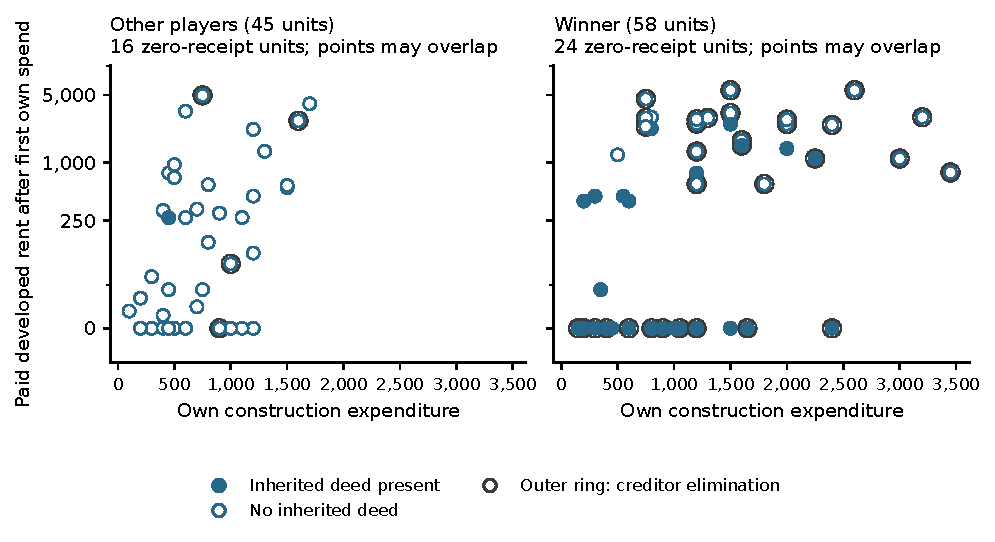
\includegraphics[width=\linewidth]{spending.pdf}
\caption{All 103 spending units, faceted by eventual winner status. Filled points contain an inherited deed at first own spending; outer rings mark an elimination triggered by rent on that group. The vertical axis is linear to 250 and logarithmic above. Forty units have zero paid developed rent. Receipts omit unpaid demands and are not net or incremental returns, and winner status is an endpoint, not a treatment.}
\label{fig:spending}
\end{figure}

Winners account for 58 of the 103 spending units. Thirty-four of those contain an inherited deed at first own spending, and thirty first became complete through an estate. A definition based only on house purchases would miss G10's winner, which inherits four-house light blues and buys \$150 of hotel conversions. The \$450 gap between whole-game and post-first-spend receipts is G2 light-blue rent collected on inherited development before the owner's first purchase.
